%\documentclass[11pt]{paper}
%\usepackage{palatino}
%\usepackage{amsfonts,amsmath,amssymb}
%% \usepackage{graphicx}
%
%
%\usepackage{listings}
%\usepackage{textcomp}
%\usepackage{color}
%
%\definecolor{dkgreen}{rgb}{0,0.6,0}
%\definecolor{gray}{rgb}{0.5,0.5,0.5}
%\definecolor{mauve}{rgb}{0.58,0,0.82}
%
%\lstset{frame=tb,
%  language=R,
%  aboveskip=3mm,
%  belowskip=3mm,
%  showstringspaces=false,
%  columns=flexible,
%  basicstyle={\small\ttfamily},
%  numbers=none,
%  numberstyle=\tiny\color{gray},
%  keywordstyle=\color{blue},
%  commentstyle=\color{dkgreen},
%  stringstyle=\color{mauve},
%  breaklines=true,
%  breakatwhitespace=true,
%  tabsize=3
%}
%
%
%\ifx\pdftexversion\undefined
%    \usepackage[dvips]{graphicx}
%\else
%    \usepackage[pdftex]{graphicx}
%    % \usepackage{epstopdf}
%    % \epstopdfsetup{suffix=}
%    \usepackage[outdir=./]{epstopdf}
%\fi
%
%\usepackage{subfig}
%
%
%\begin{document}

%%%%%%%%%%%%%%%%%%%%%%%%%%%%%%%%%%%%%%%%
% Problem Set 7
%%%%%%%%%%%%%%%%%%%%%%%%%%%%%%%%%%%%%%%%

%\pagestyle{empty}
%{\noindent\bf Spring 2021 \hfill Firstname M.~Lastname}
%\vskip 16pt
%\centerline{\bf University of Central Florida}
%\centerline{\bf College of Business}
%\vskip 16pt
%\centerline{\bf QMB 6911}
%\centerline{\bf Capstone Project in Business Analytics}
%\vskip 10pt
%\centerline{\bf Solutions:  Problem Set \#7}
%\vskip 32pt
%\noindent


% \pagebreak
\section{Analyzing the Dependent Variable}

\subsection{Probability Density Function of Fly Reel Prices}

Figure \ref{fig:density_prices} is the kernel-smoothed probability density function of the natural logarithm of
price:

\begin{figure}[h!]
  \centering
  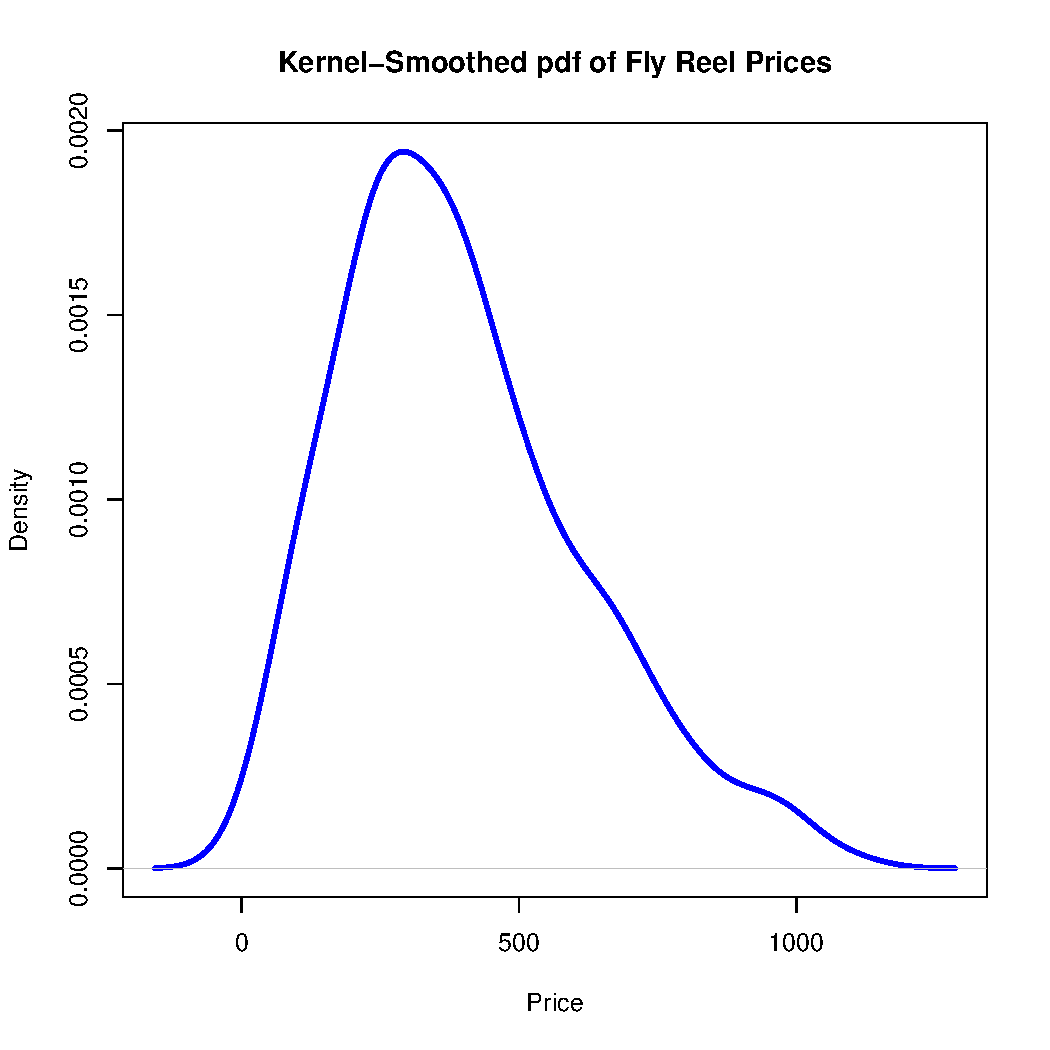
\includegraphics[scale = 0.5, keepaspectratio=true]{../Figures/density_prices}
  \caption{Probability Density Function of Fly Reel Prices} \label{fig:density_prices}
\end{figure}


\subsection{Probability Density Function of the Log. of Fly Reel Prices}

Figure \ref{fig:density_log_prices} is the kernel-smoothed probability density function of the natural logarithm of
price:

\begin{figure}[h!]
  \centering
  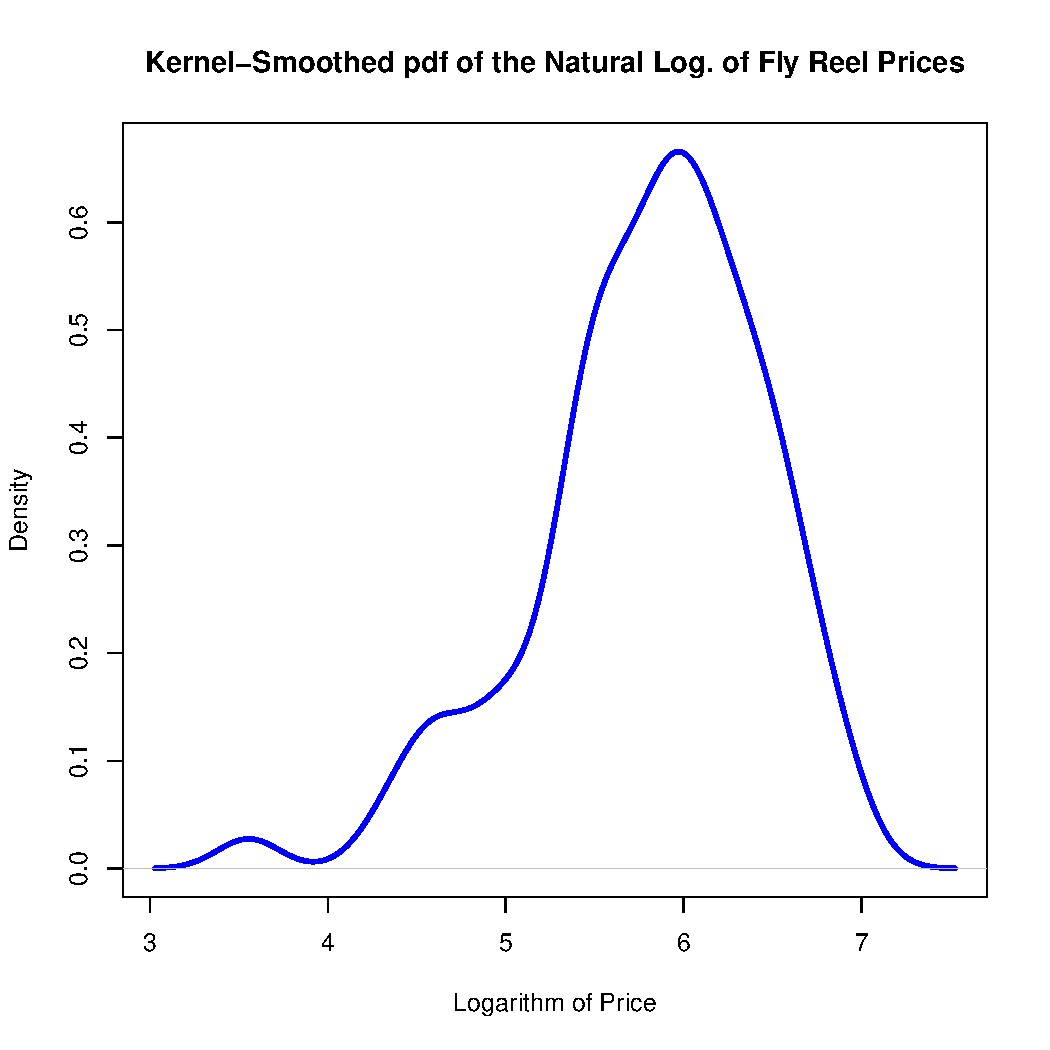
\includegraphics[scale = 0.5, keepaspectratio=true]{../Figures/density_log_prices}
  \caption{Probability Density Function of Fly Reel Prices} \label{fig:density_log_prices}
\end{figure}



\pagebreak
\subsection{Probability Density Function of the Box-Cox Transformation of Fly Reel Prices}

Figure \ref{fig:density_trans_prices} is the kernel-smoothed probability density function of the natural logarithm of
price. 
Although the transformed model does look closest to normal,
all three distributions are reasonably symmetric, 
indicating that the use of the transformation is subject to judgment.
Whether it is worth using the transformation
can be settled by analyzing the results of regression models 
with different forms of the dependent variable. 

\begin{figure}[h!]
  \centering
  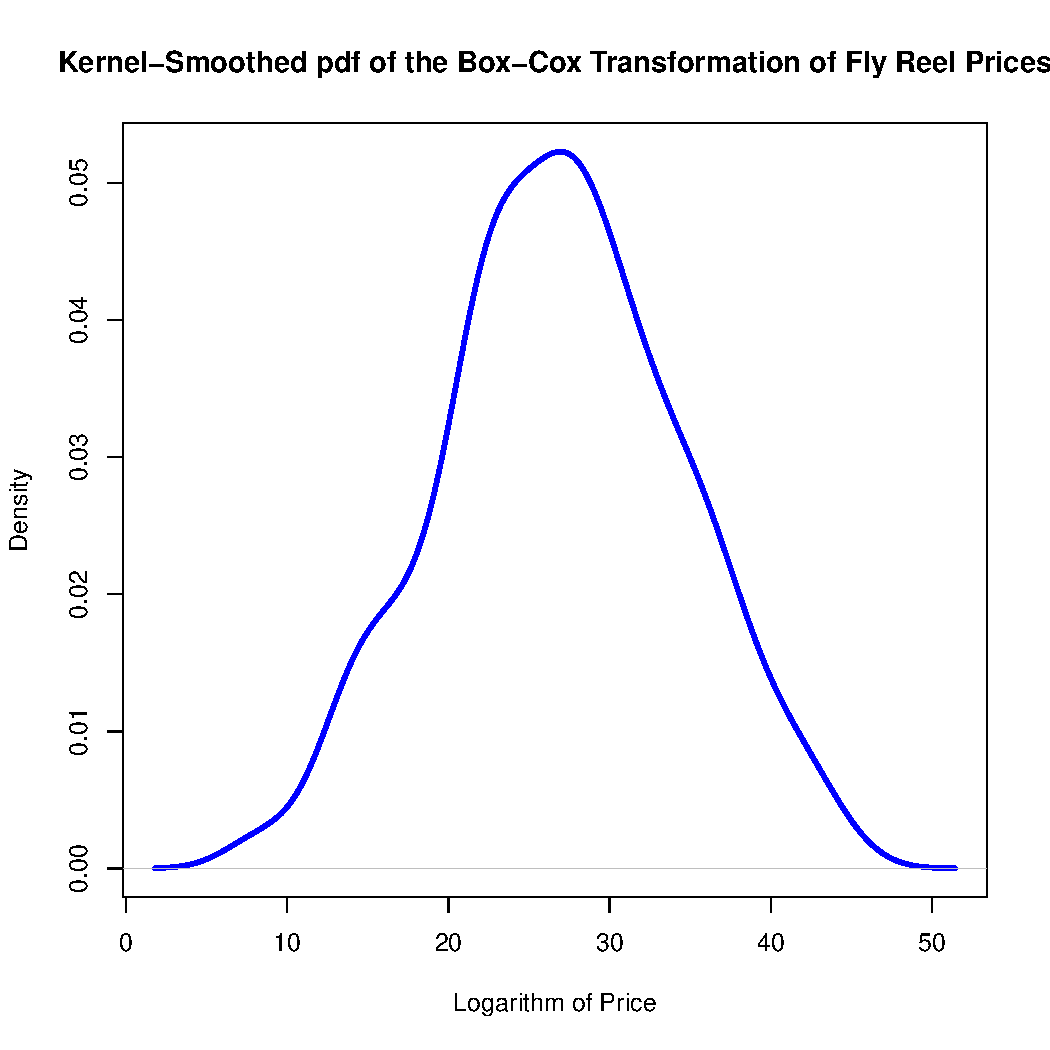
\includegraphics[scale = 0.5, keepaspectratio=true]{../Figures/density_trans_prices}
  \caption{Probability Density Function of Transformed Fly Reel Prices} \label{fig:density_trans_prices}
\end{figure}


\pagebreak
\section{Regression Models for Fly Reel Prices}


For the regression analysis, I create new variables.
The first is the volume of each reel, 
calculated as the volume of a cylinder: 
the value $\pi$ times the square of the radius of the reel,
times the width of the reel. 
The density is then calculated as the weight 
divided by the volume. 

\begin{lstlisting}[language=R]
R> flyreels[, 'Volume'] <- 
	pi * (flyreels[, 'Diameter']/2)^2 * flyreels[, 'Width']
R> flyreels[, 'Density'] <- 
	flyreels[, 'Weight'] / flyreels[, 'Volume']
\end{lstlisting}



% \pagebreak
\subsection{Comparison by Transformation of Dependent Variable}

Table \ref{tab:reg_by_dep_var} shows the results of 
a series of regression models with different definitions of the dependent variable.
Model 1 uses the fly reel prices without transformation, 
Model 2 uses the logarithm of the fly reel prices, 
and Model 3 uses the Box-Cox transformation of fly reel prices, 
with the optimal value of the parameter in the exponent.
% 
Although the model built on the original price levels
has statistically significant coefficients, 
the two transformed models have a better fit, 
with higher values of $\bar{R}^2$. 
Since the difference between the latter two models is marginal, 
it is better to model the logarithm of fly reel prices, 
which has the added advantage of interpretability 
of the coefficients, 
which approximately represent percentage changes in fly reel prices. 


\begin{table}
\begin{center}
\begin{tabular}{l c c c}
\hline
 & Model 1 & Model 2 & Model 3 \\
\hline
(Intercept)       & $-1056.01^{***}$ & $2.09^{***}$ & $-19.77^{***}$ \\
                  & $(105.51)$       & $(0.26)$     & $(3.21)$       \\
Width             & $158.71^{*}$     & $0.30$       & $4.38^{*}$     \\
                  & $(63.32)$        & $(0.16)$     & $(1.92)$       \\
Diameter          & $174.36^{***}$   & $0.40^{***}$ & $5.37^{***}$   \\
                  & $(20.59)$        & $(0.05)$     & $(0.63)$       \\
Density           & $596.81^{***}$   & $1.20^{***}$ & $17.19^{***}$  \\
                  & $(89.17)$        & $(0.22)$     & $(2.71)$       \\
SealedYes         & $144.31^{***}$   & $0.42^{***}$ & $5.00^{***}$   \\
                  & $(20.43)$        & $(0.05)$     & $(0.62)$       \\
MachinedYes       & $114.40^{***}$   & $0.76^{***}$ & $6.53^{***}$   \\
                  & $(30.43)$        & $(0.08)$     & $(0.92)$       \\
made\_in\_USATRUE & $202.10^{***}$   & $0.52^{***}$ & $6.51^{***}$   \\
                  & $(19.86)$        & $(0.05)$     & $(0.60)$       \\
\hline
R$^2$             & $0.64$           & $0.74$       & $0.71$         \\
Adj. R$^2$        & $0.63$           & $0.73$       & $0.70$         \\
Num. obs.         & $248$            & $248$        & $248$          \\
\hline
\multicolumn{4}{l}{\scriptsize{$^{***}p<0.001$; $^{**}p<0.01$; $^{*}p<0.05$}}
\end{tabular}
\caption{Regression Models with Different Dependent Variables}
\label{tab:reg_by_dep_var}
\end{center}
\end{table}


\pagebreak
\subsection{Comparison by Country of Manufacture}

Table \ref{tab:reg_by_country} shows the results of 
a series of regression models 
on different samples by country of manufacture.
Model 1 shows the results for the sample of fly reels made in the USA
and Model 2 shows the remaining fly reels made in China or Korea.


\begin{table}
\begin{center}
\begin{tabular}{l c c c c}
\hline
 & Model 1 & Model 2 & Model 3 & Model 4 \\
\hline
(Intercept) & $3.35^{***}$ & $3.48^{***}$ & $2.03^{***}$ & $2.41^{***}$ \\
            & $(0.30)$     & $(0.28)$     & $(0.47)$     & $(0.41)$     \\
Width       & $0.28$       &              & $0.39$       &              \\
            & $(0.22)$     &              & $(0.23)$     &              \\
Diameter    & $0.44^{***}$ & $0.49^{***}$ & $0.36^{***}$ & $0.41^{***}$ \\
            & $(0.07)$     & $(0.05)$     & $(0.08)$     & $(0.07)$     \\
Density     & $1.13^{***}$ & $1.06^{***}$ & $1.32^{**}$  & $1.06^{**}$  \\
            & $(0.25)$     & $(0.25)$     & $(0.41)$     & $(0.38)$     \\
SealedYes   & $0.32^{***}$ & $0.32^{***}$ & $0.65^{***}$ & $0.64^{***}$ \\
            & $(0.06)$     & $(0.06)$     & $(0.10)$     & $(0.10)$     \\
MachinedYes &              &              & $0.65^{***}$ & $0.63^{***}$ \\
            &              &              & $(0.09)$     & $(0.09)$     \\
\hline
R$^2$       & $0.54$       & $0.53$       & $0.75$       & $0.74$       \\
Adj. R$^2$  & $0.52$       & $0.52$       & $0.73$       & $0.73$       \\
Num. obs.   & $135$        & $135$        & $113$        & $113$        \\
\hline
\multicolumn{5}{l}{\scriptsize{$^{***}p<0.001$; $^{**}p<0.01$; $^{*}p<0.05$}}
\end{tabular}
\caption{Regression Models by Country of Manufacture}
\label{tab:reg_by_country}
\end{center}
\end{table}


The width of the reel is insignificant in both samples
and the coefficients are qualitatively similar across the samples, as well as matching in significance. 
This suggests that one model might be sufficient. 

To test this statistically, I conduct an $F$-test. 
This compares a single model with only an
indicator for the country of manufacture
(the restricted model)
with a separate model for each country.
In this case, the full, unrestricted model has 
$K = 2\times6 = 12$ parameters, one for each variable in two models. 
The test that all of the coefficients are the same has 
$M = 6 - 1 = 5$
restrictions. 
The one restriction fewer accounts for the made-in-USA indicator
in the full model, 
which allows for two separate intercepts. 
% 
The $F$-statistic has a value of 

$$ 
\frac{(RSS_M - RSS)/M}{RSS/(N - K - 1)} = \frac{(26.24962 - 25.2235)/5}{25.2235/235} = 1.912007. 
$$

This value is greater than 1, so we can compare it to the critical value
of the $F$-statistic at the specified degrees of freedom for
a conventional level of significance.
These critical values are 
3.095, 2.252, and 1.872
at the 1\%, 5\%, and 10\%
levels of significance, respectively.

This places the F-statistic between the critical values for the
5 and 10 percent levels of significance.
Conclude that fly reel prices may have some difference by
country of manufacture but the difference is marginal.
This suggests little justification for separate models by
country of manufacture.
We can investigate small differences between the models.


In the next section, 
I will consider a hybrid model with some interaction terms
with separate coefficients by country of manufacture. 


\pagebreak
\subsection{Models with Interaction Terms}

Table \ref{tab:reg_interactions} shows the results of 
a series of regression models with different 
specifications of interaction terms by country of manufacture. 
% 
The interaction with sealed and country of manufacture is significant in both specifications Model 1 and Model 3.
In contrast, the interaction with density was not significant. 
Furthermore, the width of fly reels is a significant predictor
in this more refined model. 
Since all variables are significant in this model and it
has the highest $\bar{R}^2$, Model 1 is the recommended model.



\begin{table}
\begin{center}
\begin{tabular}{l c c c c}
\hline
 & Model 1 & Model 2 & Model 3 & Model 4 \\
\hline
(Intercept)          & $8.89189^{***}$  & $8.88028^{***}$  & $8.87926^{***}$  & $8.89127^{***}$  \\
                     & $(0.12827)$      & $(0.11042)$      & $(0.11163)$      & $(0.11165)$      \\
horsepower           & $0.00488^{***}$  & $0.00490^{***}$  & $0.00489^{***}$  & $0.00476^{***}$  \\
                     & $(0.00039)$      & $(0.00039)$      & $(0.00039)$      & $(0.00043)$      \\
age                  & $-0.02986^{***}$ & $-0.02994^{***}$ & $-0.02990^{***}$ & $-0.02969^{***}$ \\
                     & $(0.00381)$      & $(0.00381)$      & $(0.00400)$      & $(0.00381)$      \\
enghours             & $-0.00004$       & $-0.00004^{***}$ & $-0.00004^{***}$ & $-0.00004^{***}$ \\
                     & $(0.00003)$      & $(0.00001)$      & $(0.00001)$      & $(0.00001)$      \\
diesel               & $0.28447^{*}$    & $0.30271^{**}$   & $0.29874^{**}$   & $0.29293^{**}$   \\
                     & $(0.12619)$      & $(0.10378)$      & $(0.10389)$      & $(0.10387)$      \\
fwd                  & $0.25952^{***}$  & $0.25727^{***}$  & $0.25879^{***}$  & $0.26050^{***}$  \\
                     & $(0.06238)$      & $(0.06230)$      & $(0.06229)$      & $(0.06226)$      \\
manual               & $-0.16119^{*}$   & $-0.15793^{*}$   & $-0.16018^{*}$   & $-0.16217^{*}$   \\
                     & $(0.06631)$      & $(0.06632)$      & $(0.06692)$      & $(0.06619)$      \\
johndeere            & $0.31091^{***}$  & $0.25824^{*}$    & $0.30345^{*}$    & $0.24957^{*}$    \\
                     & $(0.07868)$      & $(0.11399)$      & $(0.15228)$      & $(0.10998)$      \\
cab                  & $0.67506^{***}$  & $0.67717^{***}$  & $0.67571^{***}$  & $0.67665^{***}$  \\
                     & $(0.06732)$      & $(0.06728)$      & $(0.06734)$      & $(0.06722)$      \\
enghours:diesel      & $0.00001$        &                  &                  &                  \\
                     & $(0.00003)$      &                  &                  &                  \\
enghours:johndeere   &                  & $0.00001$        &                  &                  \\
                     &                  & $(0.00002)$      &                  &                  \\
age:johndeere        &                  &                  & $0.00023$        &                  \\
                     &                  &                  & $(0.00742)$      &                  \\
horsepower:johndeere &                  &                  &                  & $0.00057$        \\
                     &                  &                  &                  & $(0.00077)$      \\
\hline
R$^2$                & $0.77769$        & $0.77795$        & $0.77766$        & $0.77811$        \\
Adj. R$^2$           & $0.77017$        & $0.77043$        & $0.77014$        & $0.77060$        \\
Num. obs.            & $276$            & $276$            & $276$            & $276$            \\
\hline
\multicolumn{5}{l}{\scriptsize{$^{***}p<0.001$; $^{**}p<0.01$; $^{*}p<0.05$}}
\end{tabular}
\caption{Regression Models for Tractor Prices}
\label{tab:reg_interactions}
\end{center}
\end{table}



In terms of the production decision, 
there exists a substantial premium for fly reels made in the USA
but this premium is half as large for sealed reels, 
however, this reduced premium is still smaller than the 
additional value for a sealed reel.  


%%%%%%%%%%%%%%%%%%%%%%%%%%%%%%%%%%%%%%%%
% \end{document}
%%%%%%%%%%%%%%%%%%%%%%%%%%%%%%%%%%%%%%%%
